\documentclass[letterpaper,12pt]{article}
\usepackage{tabularx} % extra features for tabular environment
\usepackage{amsmath}  % improve math presentation
\usepackage{float}
\usepackage{pdfpages}

\usepackage{graphicx} % takes care of graphic including machinery
\graphicspath{ {./figures/} }
\usepackage[margin=1in,letterpaper]{geometry} % decreases margins
\usepackage{cite} % takes care of citations
\usepackage[final]{hyperref} % adds hyper links inside the generated pdf file
\hypersetup{
	colorlinks=true,       % false: boxed links; true: colored links
	linkcolor=blue,        % color of internal links
	citecolor=blue,        % color of links to bibliography
	filecolor=magenta,     % color of file links
	urlcolor =blue         
}

%
\setcounter{tocdepth}{4} 
\setcounter{secnumdepth}{4}


\begin{document}

\title{Experiment 7 \protect\\Rectifiers, Capacitors and Inductors}
\author{Ahmet Akman 2442366 \protect\\ Assistant : Uğur Berkay Saraç}
\date{\today}
\maketitle
\newpage
\tableofcontents
\newpage
%\begin{abstract}
%abstract
%\end{abstract}

\section{Introduction} 
In this experiment, as students, we are expected to experiment with rectifiers, capacitors, and inductor circuits by completing the steps described in the seventh experiment laboratory manual. The half-full rectifier circuit structures and ripple voltages are expected to be learned throughout these steps. The output versus input characteristics is observed by connecting the signal generator to the oscilloscope and the circuit. Also, the measurement techniques for the capacitance of capacitors and the inductance of inductors are expected to be expressed and experimented. The results of the steps were recorded and plotted for further comments.
\section{Experimental Results}
In this section, the results of Experiment 7 are discussed. 
\subsection{Step 1}
In this step, circuit shown in the Figure 1  is constructed. 

\section{Conclusion}

In conclusion, in experiment 7, "Rectifiers, Capacitors and Inductors," as students, we have learned how various functional circuit setups rectifiers constructed. Preliminary laboratory work is done via simulations of the rectifier, capacitor, and inductor circuits in an LTSpice environment and by mathematical relations. As students, we have seen how half-wave and full wave rectifiers behave. We have inferred the capacitance and inductance values indirectly and compared them with the direct ones. The characteristics of the q-v and \(\phi\)-i are observed with the help of their calculations. Lastly, different inductors and their behaviors are observed, and the mathematical expressions are verified via measurements. To sum up, in this experiment, as students, we have experimented with how different rectifier circuits operate, how we can measure or calculate the inductance and capacitance values. 
\section*{Appendix I}
Total time spent on/during:
\begin{itemize}
	\item Pre-lab preparation: 5 hours (including the preliminary work and simulations) 
	\item Experimental work: 2 hours (hours spent in lab)
	\item Report writing: 5 hours 
\end{itemize}
\section*{Appendix II}
The outputs of the simulations are fetched from LTSpice and plotted in MATLAB. 
%++++++++++++++++++++++++++++++++++++++++
% References section will be created automatically 
% with inclusion of "thebibliography" environment
% as it shown below. See text starting with line
% \begin{thebibliography}{99}
% Note: with this approach it is YOUR responsibility to put them in order
% of appearance.

%\begin{thebibliography}{99}

%https://tr.overleaf.com/latex/templates/sample-lab-report-for-u-of-r-phys-349/pgsyqngcyjxk

%\end{thebibliography}


\end{document}


\begin{table}[H]
	\begin{center}
		\caption{Resistance reading by color code convention.}
		\vspace{2mm}
		\begin{tabular}{||c | c | c||} 
		 \hline
		 Color Order & Value & Tolerance \\ [0.5ex] 
		 \hline\hline
		 Brown / Black / Red / Gold & 1k\( \Omega \) & \( \% \) 5  \\ 
		 \hline
		 Yellow / Violet / Red / Gold & 4.7k\( \Omega \) & \( \% \) 5   \\
		 \hline
		 Brown / Grey / Orange / Gold & 18k\( \Omega \) & \( \% \) 5  \\ [1ex] 
		 \hline
		\end{tabular}
	\end{center}
	\end{table}

	\begin{figure}[H]
 		\centering
		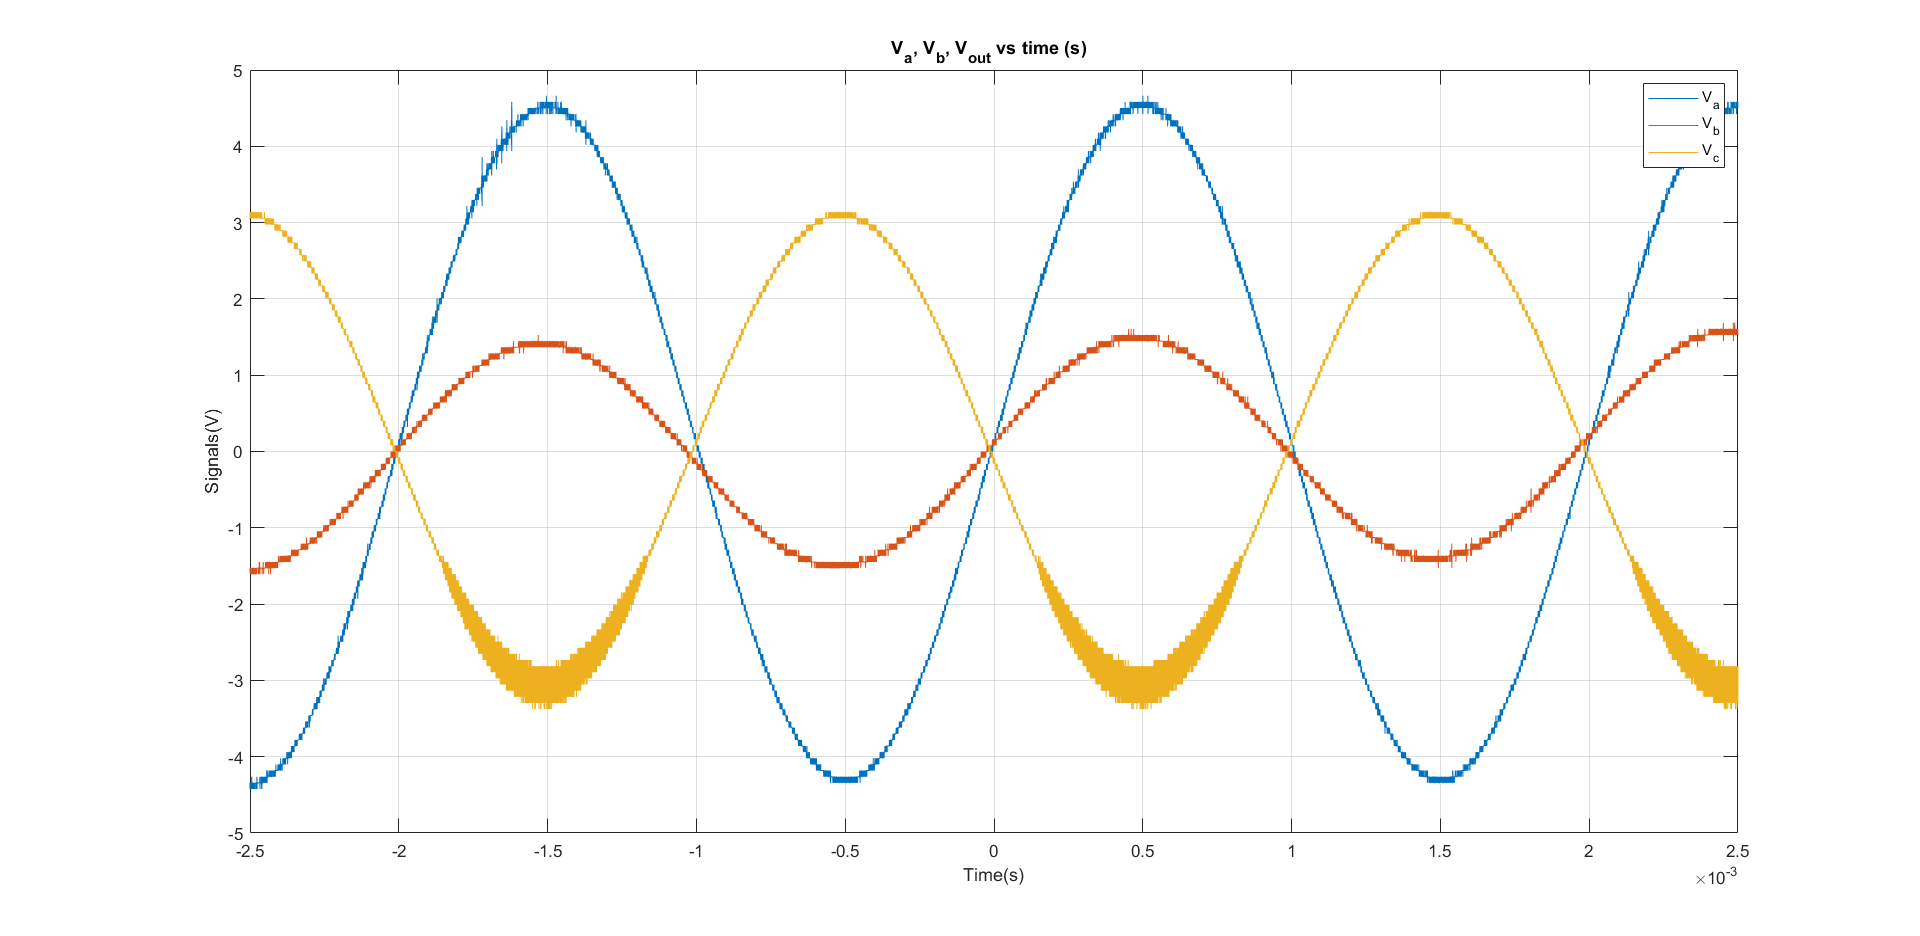
\includegraphics[width=0.6\textwidth]{5.png}
		\caption{Circuit schematic for the step 5}
	\end{figure} 

	\begin{figure}[htp] \centering{
		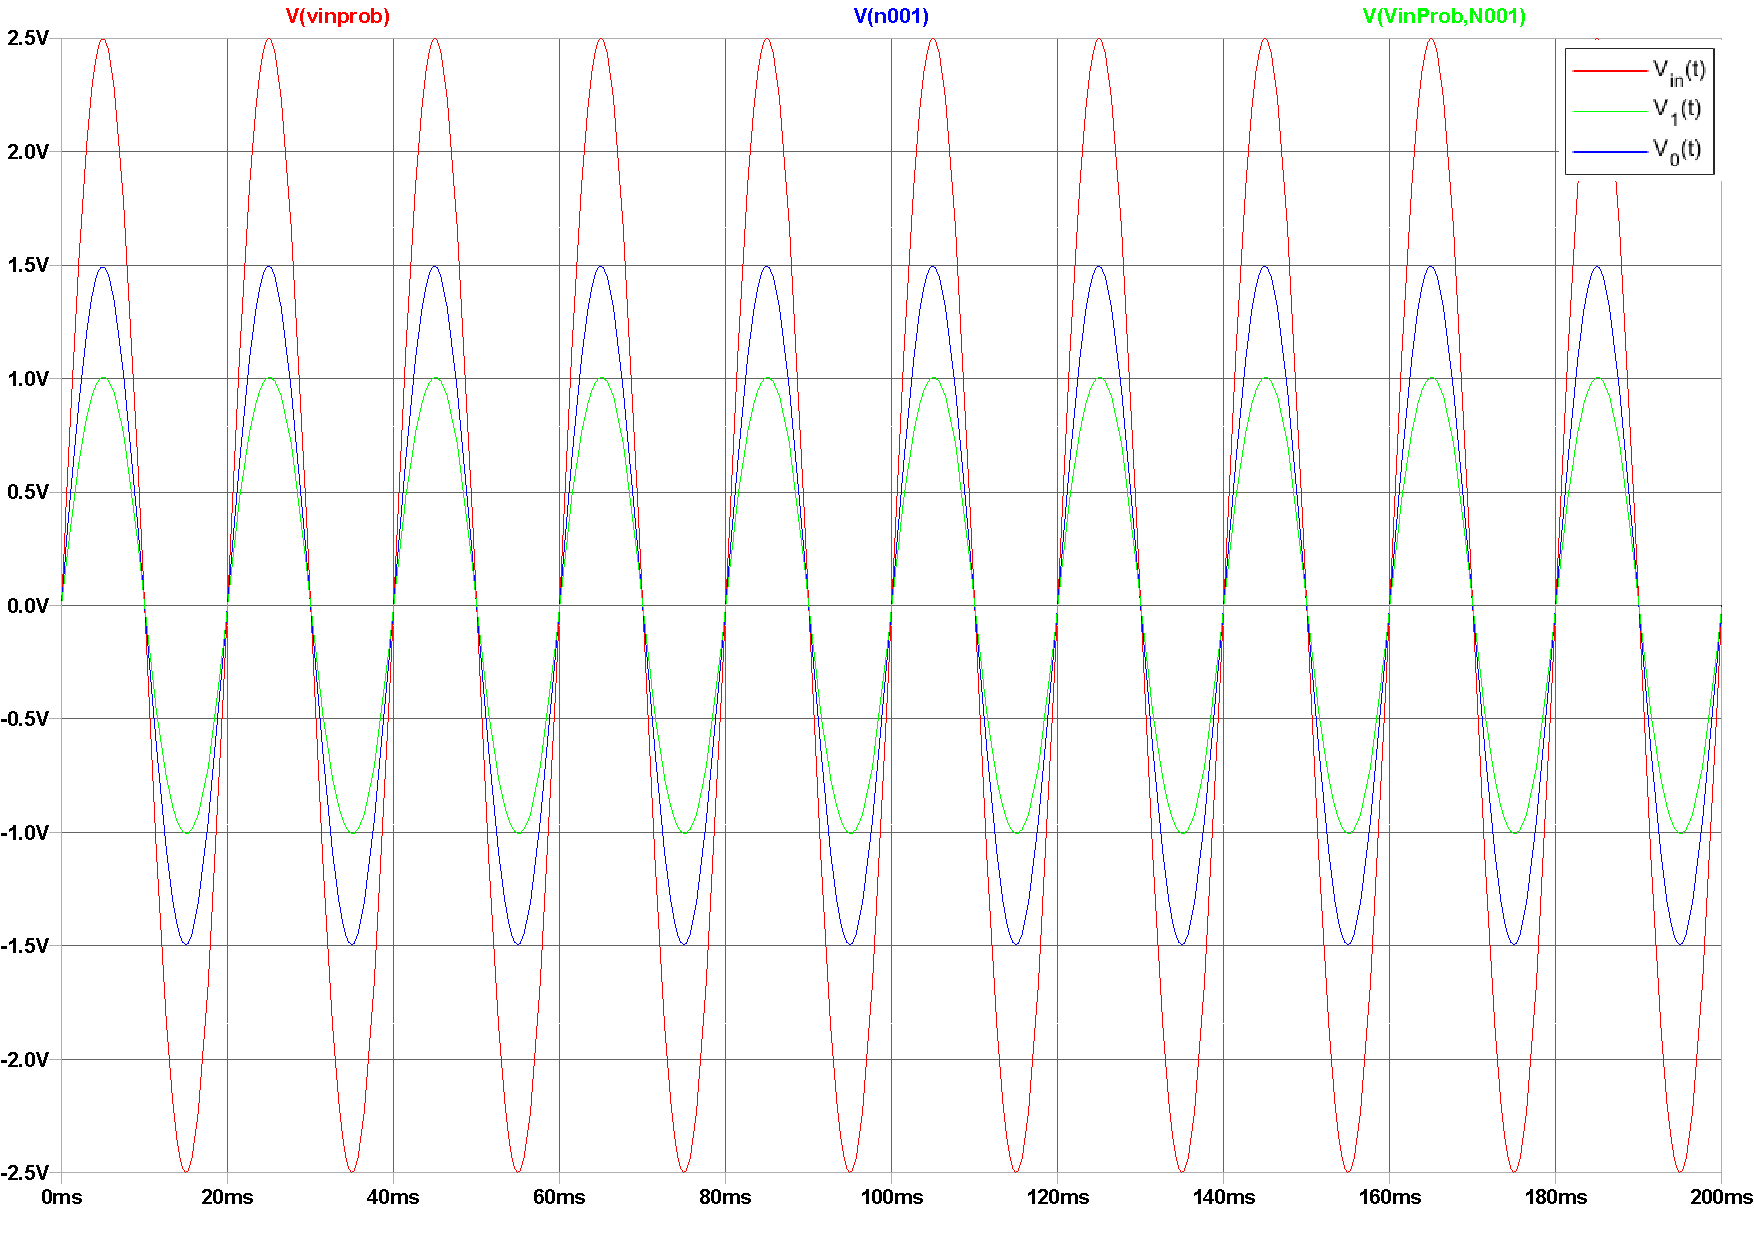
\includegraphics[scale=0.25]{2a_plot.pdf}}
		\caption{Experiment 2}
\end{figure}
	